\chapter{Introduction to Fluid-Structure Interaction}
The interaction between fluids and structures can be observed all around us in nature.
Examples of fluid-structure interaction include flags waving in the wind, windmills, and inhalation of air into the lungs. It is rather intuitive that fluids and structures must exert mutual force on each other and that the fluid and structure both can have dominant and passive properties. In the example of a flag waving in the wind, it is the forces from the flowing air that are dominant, whereas in the example of inhalation, the structure (diaphragm) is dominating. 

Understanding and modeling fluid-structure interaction (FSI) can greatly assist in design of structures such as windmill and aircraft wings. A famous example of design flaw is the collapse of the Tacoma Narrows Bridge in 1940 \cite{Billah1991}, only two months after being opened, see figure \ref{tacoma}. The bridge was literally shaken apart due to strong winds (64 km/h) interacting with the structure, making it resonate. No human lives were lost in the collapse, but a Cocker Spaniel named Tubby left behind in a car was not that lucky and lost its life in the bridge collapse. \newline

\begin{figure}
\centering
\begin{minipage}{.50\textwidth}
  \centering
  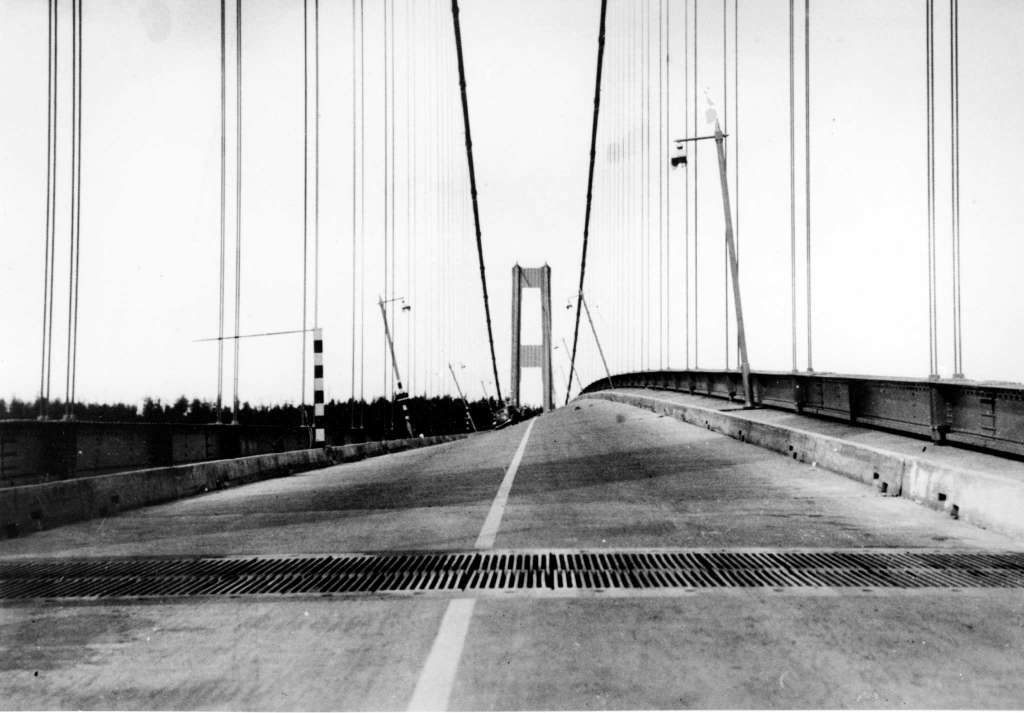
\includegraphics[width=.95\linewidth]{./IntroductionToFSI/tacoma2.jpeg}
  \label{fig:test1}
\end{minipage}%
\begin{minipage}{.50\textwidth}
  \centering
  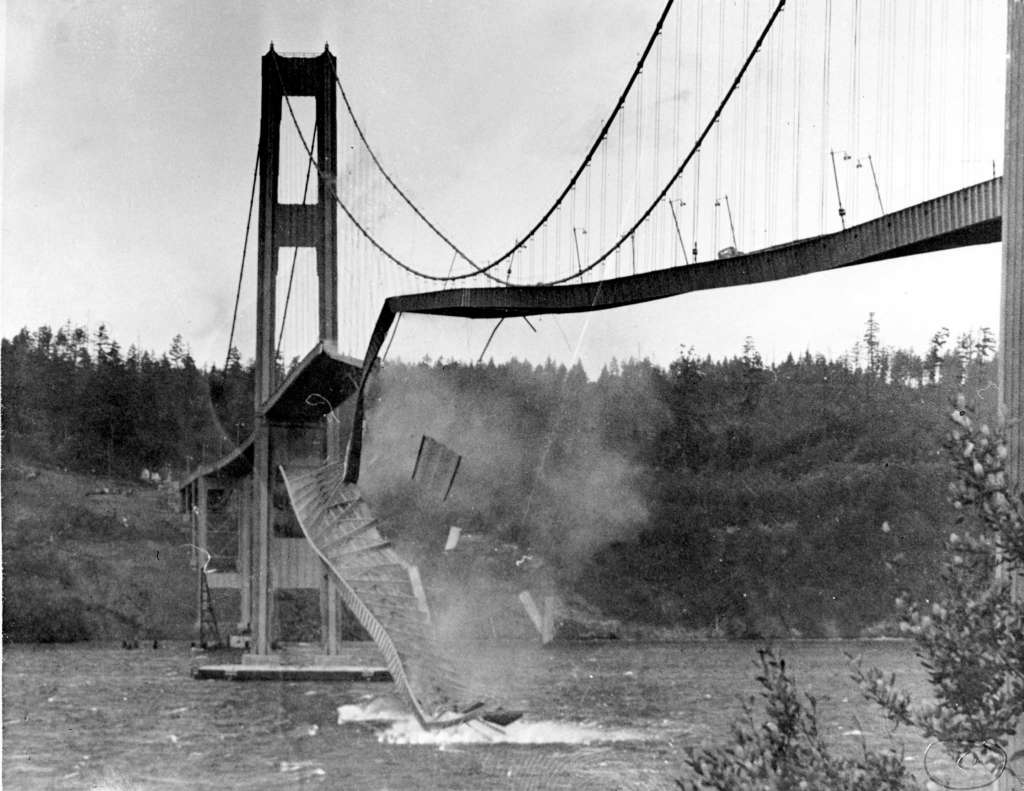
\includegraphics[width=.86\linewidth]{./IntroductionToFSI/tacoma3.jpeg}
  \label{fig:test2}
\end{minipage}
  \caption{Left: Tacoma Narrows bridge still standing with large deformations, Right: Tacoma Narrows bridge collapsed}
  \label{tacoma}
\end{figure}

FSI has matured and is now routinely used to model and design the motion and wakes of windmills.
Since there is a big difference in density between fluid and structure $\frac{\rho_f}{\rho_s} << 1$, the structural deformations are small and the interaction is \say{easy} to model. However, modeling arterial FSI deems more challenging as the density of the fluid (blood) and the structure (artery) are similar, resulting in large deformations of the arteries. Large deformations are challenging to model and require hyperelastic constitutive laws, and energy stable numerical schemes.\newline

A scientific branch of fluid mechanics is Computational Fluid Dynamics, where computers and numerical algorithms are used to solve fluid problems. Similarly, a name used for solving fluid-structure interaction problems is simply \say{FSI}. However, it should be emphasized that it is actually \textit{Computational Fluid Structure Interaction} (CFSI) that will be addressed in this thesis. The same name applies to the word \say{Structure} where the actual problem to be solved belongs to the scientific branch of solid mechanics. \newline

The goal of this master thesis is to develop a computational framework to solve FSI problems arising in biomechincs, namely large deformations. The effects of different numerical schemes and approaches will be investigated to maintain acceptable accuracy.



\begin{comment}
Fluid-Structure Interaction problem can be observed all around us in nature, from large industrial engineering complexes to the smallest blood vessels in the human body. A large scale example is the collapse of the Tacoma Narrows Bridge that collapsed in 1940 only two months after being opened. The collapse was due to aero-elastic fluttering from strong winds. No human life was lost in the collapse, but a cocker spaniel name Tubby left in a car was not so lucky. The construction of windmills are a second example of the Fluid-Structure Interaction problem. Todays windmills are rigid and hence giving a big difference in density between fluid and structure, $ \rho_s >> \rho_f $. The structure will therefore only give rise to small deformations. However applying FSI to hemodynamics( dynamics of blood flow ) deems more challenging. One FSI hemodynamic problem are inter-cranial aneurysms, which are balloon shaped geometries often occurring where a blood vessel splits into two parts, due to weak vessel walls. Bursting of one of these aneurysms in the skull can have fatale consequences. With fluid and structure densities more equal than the previous example, the structure has an elastic character giving under the right circumstances large deformations. The blood flow also transitions to turbulent flow. This combination gives the need for a rigid stabile solver. Therefore the main goal of this master thesis is to build a framework to solve the FSI problem, investigating different approaches and schemes. The framework will be validated and verified using MMS, companying a wide range of benchmarks.  
\end{comment}

